\documentclass{article}

\usepackage{graphicx} % Required for inserting images
\usepackage{listings}
\usepackage{color}

\definecolor{dkgreen}{rgb}{0,0.6,0}
\definecolor{gray}{rgb}{0.5,0.5,0.5}
\definecolor{mauve}{rgb}{0.58,0,0.82}

\lstset{frame=tb,
  language=Bash,
  aboveskip=3mm,
  belowskip=3mm,
  showstringspaces=false,
  columns=flexible,
  basicstyle={\small\ttfamily},
  numbers=none,
  numberstyle=\tiny\color{gray},
  keywordstyle=\color{blue},
  commentstyle=\color{dkgreen},
  stringstyle=\color{mauve},
  breaklines=true,
  breakatwhitespace=true,
  tabsize=3
}

\title{HW07}
\author{Riccardo Zucchelli 1984963}
\date{December 2024}

\begin{document}

\maketitle

\section*{Introduction}
In this homework we will be talking about TLS, the use of \texttt{openssl s\_client} to test them, and it's implementation throughout a list of popular websites.
\subsection*{Transport Layer Security}
Transport Layer Security, or TLS in short, is a widely adopted security protocol designed to facilitate privacy and data security for communications over the Internet. A primary use case of TLS is ensuring encryption, by hiding the communication between web applications and servers, such as web browsers loading a website, integrity of the server and authentication of it and so greatly mitigating attacks based on identity forging. It's greater use was to superseed the use of the old HTTP web standard, which wasn't designed by any sort of security in mind; this meant that anyone could sniff open traffic and capture sensitive data, fake it's identity or do phishing. It was proposed by IETF in 1999 as the evolution to the Netscape Secure Socket Layer, or SSL, and got few revisions until the publishing of TLS 1.3 in 2018.
The use of TLS certificates creates a chain of trust that can be completely verified up until the Root CA, which means that the identity of the website has been digitally signed by a trusted party.

Throughout all of its revisions, from TLS 1.0 up until TLS 1.3 there has been some major updates both in terms of security and in efficiency. Even if most websites aren't using the latest revision, and keeping TSL 1.2, they can be overall considered safe, although slower than their TLS 1.3 counterparts, if weak cyphers and algorithms aren't accepted. The handshake differences can be seen in the Figure \ref{fig:tls_diff}

We'll be using openssl, specifically it's \texttt{s\_client} toolchain to verify the supported TLS version of some websites and evaluate their security.
A great website should be having TLS 1.3, and not accept anything below 1.2, but we will consider a pass in security if TLS 1.2, which is widely supported even on legacy hardware, is the accepted protocol, and the completely broken TLS 1.1 and TLS 1.0 aren't.
\begin{figure}
    \centering
    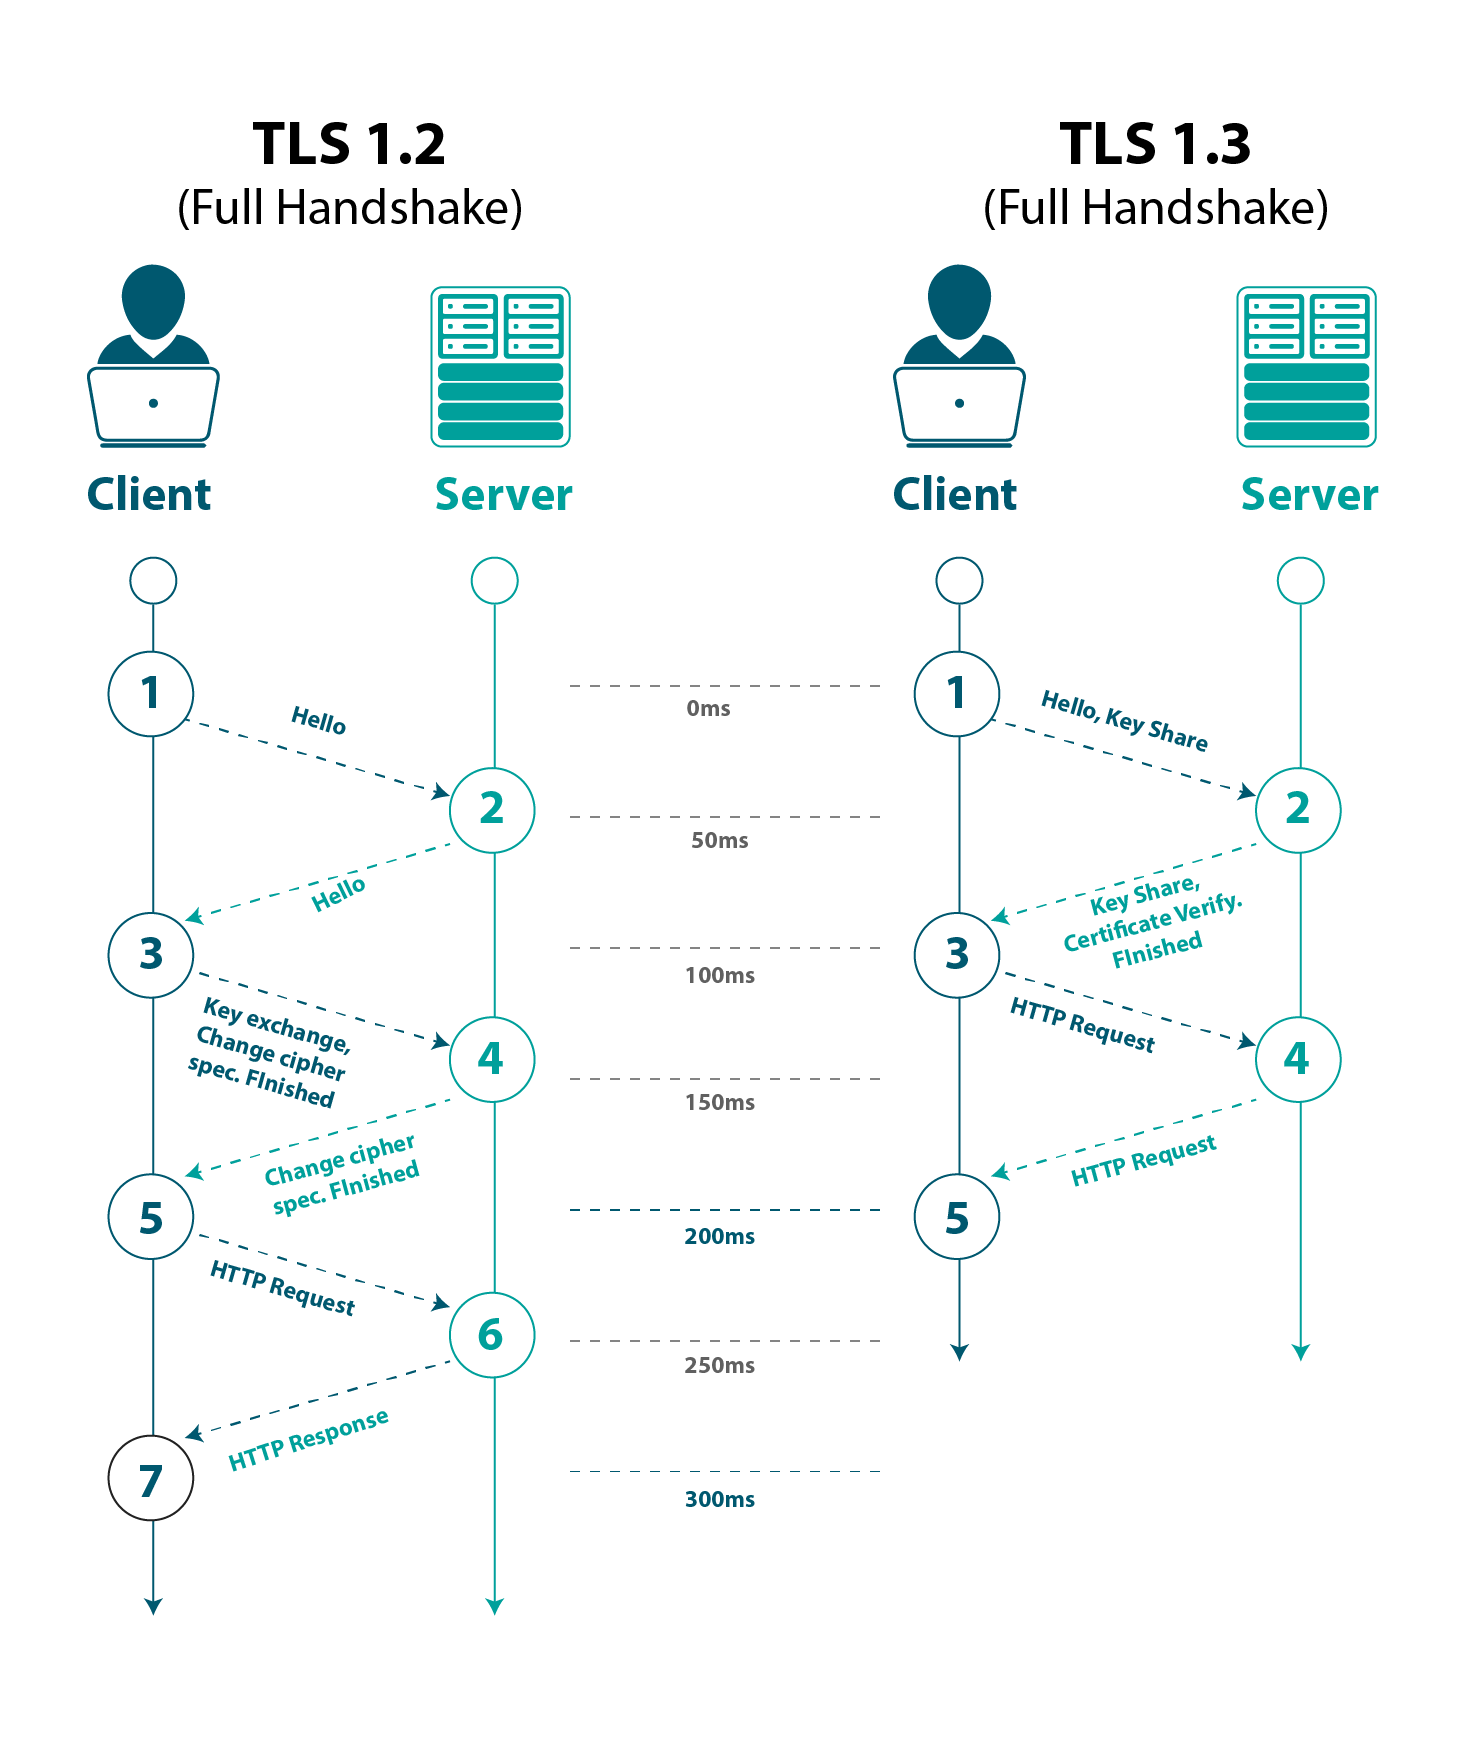
\includegraphics[width=0.6\linewidth]{tls_diff.png}
    \caption{Differences between TLS 1.3 and TLS 1.2}
    \label{fig:tls_diff}
\end{figure}

\section*{Website testing}
By using websites that analyze user traffic we'll consider some of the most popular websites visited in Italy, along with websites more tailored to people in Tech. For example, we'll be visiting websites such as:
\begin{itemize}
    \item google.com
    \item corriere.it
    \item github.com
    \item twitter.com
    \item repubblica.it
\end{itemize}
Every website listed here is included in the \texttt{websites} list variable in the code \ref{code:tls_test} below. We'll also see if any of these websites allow clients requesting the use of TLS 1.1 and below by using \texttt{-tls1\_x} directive.

On figure \ref{fig:websites} we can see how the tested websites did, and overall every one passed our security test. We can see some interesting patterns arise: although everyone supported TLS 1.2, most of
the Italian websites didn't support the newest revision.
This is not a problem, but in CS Security we can absolutely say that something \textit{is very safe, until it isn't}, and most of Internet Security is based on computational difficulty. Once computers become faster and faster, while being on the edge of a \textit{quantum boom}, old standards become deprecated. This means that there is a very good reason to always stay updated on the newest security protocol standards.


\begin{figure}
    \centering
    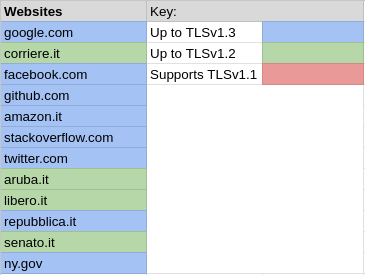
\includegraphics[width=0.6\linewidth]{websites.png}
    \caption{Websites tested}
    \label{fig:websites}
\end{figure}

\section*{Time Test}
After eliminating the outliers, the comparison between TLS 1.3 and TLS 1.2 handshake times reveals a clear performance advantage for TLS 1.3. The handshake times for TLS 1.3 are noticeably shorter, with some instances being up to 2x faster than their TLS 1.2 counterparts.

When visualizing the data with a horizontal histogram, it becomes evident that TLS 1.3 handshakes are generally quicker, and it's time difference can be attributed to a more efficient handshake (as also discussed before and shown in the Figure \ref{fig:tls_diff}).
\begin{figure}
    \centering
    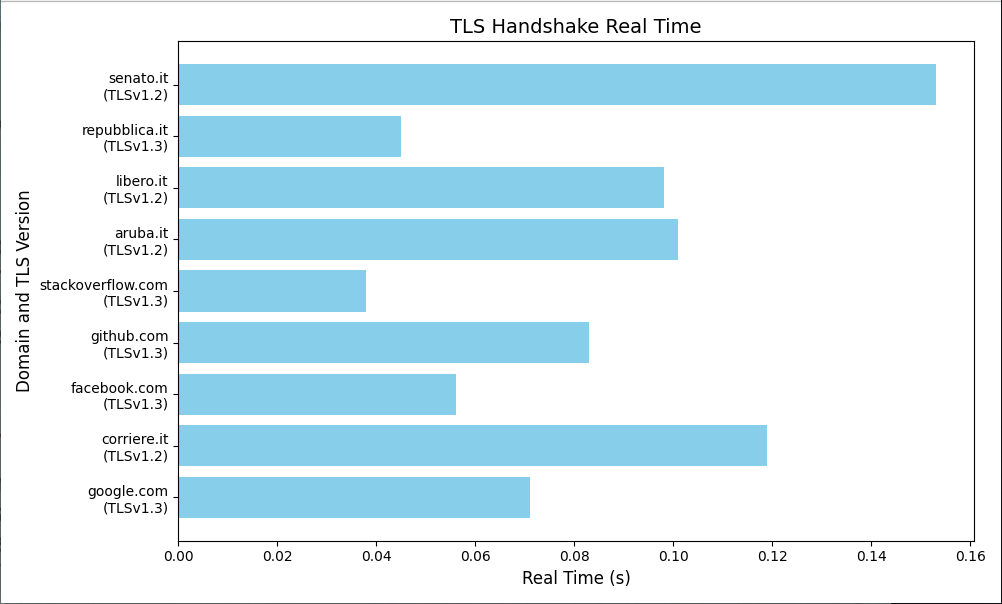
\includegraphics[width=0.8\linewidth]{time.png}
    \caption{Time tested on Real Time}
    \label{fig:time}
\end{figure}

\section*{TLS-Based attacks}
The use of TLS 1.1 on modern servers poses significant security risks. As a deprecated protocol, it lacks the robust cryptographic protections offered by more recent versions, such as TLS 1.2 and TLS 1.3. A server that accepts TLS 1.1 sessions is vulnerable to known attacks, including \textit{BEAST} (Browser Exploit Against SSL/TLS), which exploits predictable initialization vectors in CBC (Cipher Block Chaining) mode, allowing attackers to decrypt sensitive data such as session cookies or login credentials during transit. 

Moreover, the presence of legacy protocol support increases susceptibility to \textit{downgrade attacks}, such as the \textit{POODLE} (Padding Oracle On Downgraded Legacy Encryption) attack. In this attack, an adversary can manipulate the handshake process to force a connection to use the older, less secure TLS 1.1 (or even SSL 3.0), enabling them to exploit vulnerabilities that could also downgrade a HTTPS session to an HTTP one.


\newpage

\subsection*{Code used}

\begin{lstlisting}[language=bash]
#!/bin/bash

# List of websites to test
websites=(
    "google.com"
    "corriere.it"
    "facebook.com"
    "github.com"
    "amazon.it"
    "stackoverflow.com"
    "twitter.com"
    "aruba.it"
    "libero.it"
    "repubblica.it"
)

# Function to test TLS handshake time
test_tls_handshake() {
    local website=$1
    echo "Testing TLS handshake for $website..."

    # Run s_client to initiate TLS handshake and capture time
    time echo | openssl s_client \
        -connect "$website":443 \
        -servername "$website" \
        -brief # removes the headache of filtering out TLS Certificate
}

# Loop through all the websites
for website in "${websites[@]}"; do
    test_tls_handshake "$website"
done
\end{lstlisting}\label{code:tls_test}

\end{document}
